\documentclass[10pt]{report}
\usepackage{tikz}
\usetikzlibrary{arrows}
\usepackage{natbib}
\usepackage{graphicx}
\usepackage{url}
\usepackage{fancyhdr}
\pagestyle{fancy}

\lhead{CAPTools Documentation}
\rhead{KU System-Level Design Group}
\lfoot{\copyright The University of Kansas, 2019}
\cfoot{\thepage}

\newtheorem{conjecture}{Conjecture}
\newtheorem{obligation}{Obligation}
\newtheorem{definition}{Definition}

\usepackage[textsize=tiny]{todonotes}
%%\usepackage{ifthen}
% \newboolean{submission}  %%set to true for the submission version

\newcommand{\squash}{\itemsep=0pt\parskip=0pt}

\parskip=\medskipamount
\parindent=0pt

\bibliographystyle{abbrvnat}


\title{Certified Attestation Protocol Tools - Version 0.1}
\author{Anna Fritz \\
  Information and Telecommunication Technology Center \\
  The University of Kansas \\
  \url{arfritzz@ku.edu}
}

\begin{document}

\chapter {Design}

\section {Initial Overview}

Negotiation occurs between two parties: the appraiser and the target.
The goal is to gather evidence about a target. The appraiser sends the
target a \textbf{request}. The target then responds
with a \textbf{proposal} which is a set of \textbf{protocols}.

\section {Basics}

To begin constructing the language, there are basic things we must implement. 

\begin{itemize}
\item Place
	\begin{itemize}
	\squash
	\item Necessary to understand where the Negotiation is taking place.
	\item Maybe place will be specialized for both the appraiser and
          the target but that is a question for later
	\item For now, place is a natural number that represents where the
          Negotiation is occurring.  
	\end{itemize}
\item Term
	\begin{itemize}
	\squash
	\item A term is a Copland term. 
	\item This is useful for the Privacy Policy to decide what terms can
          be shared. 
	\item A Proposal will be composed of a list of terms from the target
          to the appraiser.
	\item I suppose when we go to define an ordering to establish a meet
          and join we will order the terms. This seems like a natural place
          to establish ordering. 
	\end{itemize}
\item Request
	\begin{itemize}
	\item A request asks the target for evidence. 
	\item It can ask for one thing, one thing or the other thing, or
          both things. 
	\item Request is an Inductive definition then so that the constructors
          can be `one` `prod` `sum`.
	\end{itemize}
\item Proposal
	\begin{itemize}
	\item Proposal is a definition (function) which takes a request
          and generates a list of terms
	\item Somewhere somehow the privacy policy must be satisfied. 
	\item Dr. A suggest making a theorem that says "forall protocols,
          the privacy policy is satisfied"
	\item This leads me to ask "How do we write the privacy policy in
          terms of code?"
	\end{itemize}
\item What that Appraiser is willing to accept?
	\begin{itemize}
	\item The target might not respond with exactly what the appraiser
          had asked for. What is the procedure in that case?
	\item Do we accept other things? Or only what is specifically asked for?
	\item Somewhere their might be a flag that states if ONLY exact is
          acceptable but otherwise, the appraiser must list what is acceptable. 
	\end{itemize}

\end{itemize}

Knowing these pieces are needed, an initial step by step procedure can be composed.
\begin{enumerate}
\item A Request is generated from the appraiser and sent to the target
	\begin{itemize}
	\item Request now only composed of one thing.
	\end{itemize}
\item The target looks at the request and responds with the proposal. The
        proposal is a list of protocols. 
\item The appraiser selects a protocol.
\item The protocol is sent to the Attestation Manager.  
\end{enumerate} 

\begin{figure}[hbtp]
  \centering
  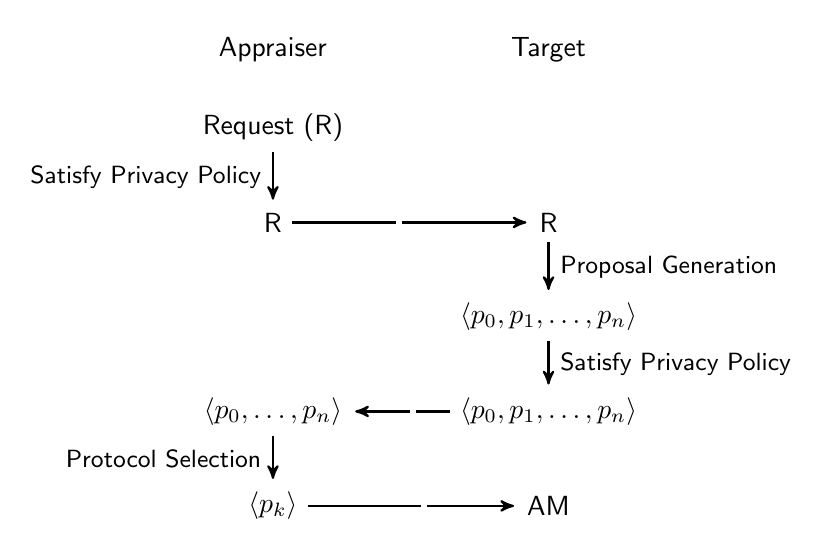
\begin{tikzpicture}[->,>=stealth',shorten >=1pt,auto,node distance=1.2cm,
  thick,main node/.style={rectangle,%%fill=blue!20,draw,
    font=\sffamily,minimum height=2mm,minimum width=2mm}]


  \node[main node] (Request) {Request (R)};
  \node[main node] (AppPrivPol) [below of=Request] {R};
  \node[main node] (R) [node distance=3.5cm, right of=AppPrivPol] {R}; 
  \node[main node] (TarPrivPol) [below of=R] {$\langle p_0,p_1,\ldots,p_n\rangle$}; 
  \node[main node] (TarProp) [below of=TarPrivPol] {$\langle p_0,p_1,\ldots,p_n\rangle$};  
  \node[main node] (AppProp) [node distance=3.5cm, left of=TarProp] {$\langle p_0,\ldots,p_n\rangle$};
  \node[main node] (Protocol) [below of=AppProp] {$\langle p_k\rangle$};
  \node[main node] (AM) [node distance=3.5cm, right of=Protocol] {AM}; 
  \node[main node] (IN) [node distance=1.0cm, above of=Request] {Appraiser};
  \node[main node] (OUT) [node distance=3.5cm, right of=IN] {Target};
    

  \path[every node/.style={font=\sffamily\small, fill=white,inner sep=1pt}]
    (Request) edge node[left=1mm] {Satisfy Privacy Policy} (AppPrivPol)
    (AppPrivPol) edge node[left=1mm] {} (R)
    (R) edge node[right=1mm] {Proposal Generation} (TarPrivPol)
    (TarPrivPol) edge node[right=1mm] {Satisfy Privacy Policy} (TarProp)
    (TarProp) edge node[right=1mm] {} (AppProp)
    (AppProp) edge node[left=1mm] {Protocol Selection} (Protocol)
    (Protocol) edge node[right=1mm] {} (AM)	
	;
\end{tikzpicture}

%%% Local Variables: 
%%% mode: latex
%%% TeX-master: "certification"
%%% End:

  \caption[Attestation and Appraisal Sequence for One Request]{Processing sequence for
    Negotiation, Selection, Attestation and Appraisal during remote
    attestation.}
  \label{fig:att-app-seq}
\end{figure}

\section {Privacy Policy}

At this point, the privacy policy is some large, overarching being
that controls the data that is sent back and forth between the appraiser
and the target. Both the appraiser and the target have their own, unique
privacy policies. Also, in more general terms, each computer or cluster
must have a privacy policy as a target and as an appraiser so that it
can morph between the two roles. 

Who communication will occur between, be it a network of computers or
one single computer, will be established in the Security Association.
Once that is established, the privacy policy may change to reflect
the communication. 

\section {Ideal trust establishment function}

The ideal trust establishment $\delta_m:R\rightarrow (E,\preceq,\top,\bot)$ ,
or delta_m. 

$\delta_m$ relates a request to the set of all evidence packages that 
could result from that request.  Those evidence packages are ordered
by $\preceq$ that defines relative``quality'' of evidence.  If
$e_1\preceq e_2$ then evidence $e_2$ is of higher quality than $e_1$.
Quality is subjective and this order reflects situational awareness.
The relation $\preceq$ is by definition a partial order 
over evidence while $\bot$ and $\top$ are the worst and best evidence
corresponding to no description and an exact description
respectively.  This defines a bounded lattice, however more work is
needed to establish the correctness of the approach.

$\gamma_n$ produces a proposal $\langle p_0,p_1,\ldots,p_n\rangle$
from a request, $r$ based on target policy. $\delta_c$
transforms the proposal into evidence from each protocol,
$\langle e_1,e_2,\ldots,e_n \rangle$. Thus $\delta_c$ is a functor
over proposals---vectors of protocols---to vectors of evidence.
$\alpha_n$ lifts the evidence vector into the evidence lattice.

\section {Request}

\subsection {Certificate Authority}
  
  As part of ISAKMP, a certificate authority is needed for strong 
  authentication of a communicating peer (ie the appraiser and the
  target). 

\subsection {Request Composition}
  
  Right now the exact understanding of the Request is not important.
  Only a general understanding in needed and useful. 
  
  A request is composed of some sort of evidence. It can be three things:
  \begin{enumerate}
  \squash
  \item one evidence
  \item sum of evidence (OR)
  \item product of evidence (AND)
  \end{enumerate}

  
  At this point, there really is not much else that is needed for a
  Request; all that is needed is evidence. In the future, some things
  that should be considered in the request are:
  
  \begin{itemize}
   \squash
   \item place
   \item the appraiser privacy policy
   \item ISAKMP
  \end{itemize}

\section {Proposal}

\subsection {Producing a proposal}

A proposal is a set of protocol generated by the target upon receiving
the target's request. Therefore, the proposal takes in the appraiser's
request and returns a list of terms. The coq definition for this may
look something like an is considered an interpreter: 
  
  \begin{verbatim}
  Definition propose : (request ev) -> list term
  \end{verbatim}  
  
  In this definition, the appraiser receives a list of terms. The list
  of terms must satisfy the privacy policy for the target before being
  sent to the appraiser. In the future, some things that should be
  considered in the proposal are:
  
  \begin{itemize}
   \squash
   \item the target's privacy policy
   \item ISAKMP
  \end{itemize}
  
  The proposal can be ordered or unordered, it does not really
  matter. The appraiser decides the ordering so the appraiser orders
  the set before selection.  

\section {Selecting Proposal}

  The function, ($\gamma_{n}$), selects a protocol (P_{k}) 
  from a proposal $\langle p_0,p_1,\ldots,p_n\rangle$.  

  The selection of a Proposal will involve ensuring that the chosen
  protocol meets the initial negotiation condition. This can be
  represented in an Inductive definition as follows:
  
  \begin{verbatim}
  Inductive negotiationR : Request -> Place -> term -> Prop :=
  | n1 : (ev1) -> n -> (USM 1) -> True
  .
  .
  .
  . where one can list various options for negotiation. 
  \end{verbatim} 
  
  The selection of a proposal has been greatly discussed. The
  appraiser will always select the proposal, but how? There must be some
  type of ordering on the members of the set that established a notion of
  "best." This is how a lattice comes into play. Within a lattice, the is
  some sort of ordering. Therefore, each unique system will produce its own
  notion of ordering allowing for there to then be a best and worst protocol
  in each set. 
	
  The lattice definition is tricky because we cannot list out cases as
  seen in the example because each system is different. Instead, we must
  keep it more general. 

\section {Evaluating Proposal}

Evaluating a proposal will occur in the Attestation Monad. The job of
Negotiation is simply to choose a protocol that will be evaluated. It is
important to note, however, the result of evaluating a proposal is evidence
about the system.  

\section {How ISAKMP fits} 

In general, Internet Security Association and Key Management Protocol
(ISAKMP) is the protocol that establishes Security Associations
(SA) and cryptographic keys outlined in RFC 2408. There are
four main goals of ISAKMP which include authenticating a communicating
peer, creation and management of security associations, key generation techniques,
and threat mitigation.

In terms of authenticating a communicating peer, ISAKMP encourages
strong authentication through the use of a certificate authority. The procedure
outlined in ISAKMP allows an entity's initial
communications to indicate which certificate authorities (CAs) it supports.
In creating and managing the security association, one side must assume the role
of initiator and the other assumes the role of responder. Proposal and
transform payloads are then exchanged to establish the security associaiton.
Also, ISAKMP provides key generation techniques that enforce  authentication
of key exchange, key exchange symmetry and perfect forward secrecy. The specifics
of key generation and transport is outlined in IKE. Finally, ISAKMP enforces
threat mitigation techniques by addressing the prevention of possible attacks
such as anti-clogging, connection hijacking, and man-in-the-middle attacks.

There are a few other concepts from ISAKMP that are important to note.
First, and entity's name is its identity where the agreed upon certificate
authority defines the naming semantics. Once the certificate the verified,
the name is verified, and then the name has meaning within the
certificate authority. Also, the domain of interpretation (DOI) defines the
situation and set of security policies that may be suppored. It also houses
additional exchange types, a scheme for naming security-relevant information,
key exchange algorithms, security policy attributes, and certificate authorities. 

\section {Questions:}
\begin{enumerate}
  \item What does the certificate authority get us? A secure channel but 
        does it say anything about the appraiser or target's
        privacy policy?
  \item How does the request generate a proposal? 
  \begin{itemize}
    \item Could think of a request as a condition like all even numbers.
    \item Then Proposal consists of many different sets composed of even
          and odd numbers with each set having varying amounts of numbers.
    \item Then what filters the set to include only even numbers?
          Is that $\delta_c$?
    \item $\delta_c$ is a functor that transforms proposals into evidence.
          I don't really understand this at all.  
  \end{itemize}
  \item Is the targets response, the proposal, an ordered list?
        I think we need a function to ensure ordering.
\end{enumerate}

\section {Examples}

Throughout the process of understanding negotiation, there are many
examples that have helped me get a better grasp on Coq and what Negotiation
entails. 

\subsection {The Fruit Example: understanding constructing values}

Let Fruit be a set such that Fruit = { apple , orange , pear }. Then an
inductive data structure for Fruit could read:  

\begin{verbatim}

Inductive request : Type := 
 | one n -> fruit
 | prod fruit -> fruit -> fruit
 | sum fruit -> fruit -> fruit.
\end{verbatim}

Where prod is equivalent to the boolean condition AND and sum is equivalent
to the boolean condition OR. Then creating examples of this would look like: 


(one apple)

(prod (one apple) (one pear))

(sum (one apple) (one pear))

(prod ((prod (one apple) (one pear)) one apple)


Therefore, one apple is a constructing value. It creates a new element that is
now part of the data structure. Overall, this Inductive definition of Request
is a "little language."

Then, generalizing this to all data type we consider the problem of wanting
to use the request data struct for a McDonald's order. If the structure was
untyped, then one could just request an order. To do this, implement the
following structure. 

\begin{verbatim}
Inductive request (ev : Type) : Type :=
| one n -> ev
| prod ev -> ev -> ev
| sum ev -> ev -> ev

\end{verbatim}


\chapter {Verification}

\section {Introduction to the formal Verification of Negotiation}

Before constructing the negotiation procedure, formal verification must occur
to ensure the process achieves the desired results. That is, that the Target
and the Appraiser's privacy policy is met and that the negotiation policy
produces an acceptable protocol for attestation. For negotiation, the architecture
design follows a specific procedure that differs from the systems verification
procedure. This is because the implementation of negotiation will differ from the
verification of negotiation. The procedure for the system's implementation can
be seen in the following list below. 

\begin{enumerate}
\item A request is sent by the Appraiser to the Target. The request must not
  violate the Appraiser's privacy policy. More detailed information about the
  Request can be found in the earilier section. 
\item The Target receives the request and generates a set of protocols also
  known as a proposal. Each protocol must satisfy the Target's privacy policy
  for each Request. 
\item The proposal is sent from the Target to the Appraiser.  
\item The Appraiser orders the set of protocols and chooses the "best" protocol.
  Multi-step negotiation may also occur but that will be discussed later. 
\item The Appraiser sends the "best" protocol through attestation where the
  protocol generates evidence about the system. 
\end{enumerate}

Before the architecture is enforced, there must be formal verification of the
negotiation system. This ensures the procedure is sound and complete. More
importantly, through verification, a notion of "best" protocol is able to be
developed and understood. The verification diagram, as seen below, details
the entire system certification from negotiation through attestation. However,
the concern here is with verification of the negotiation procedure. The
following steps, as outlined below, detail how verification of negotiation
will be accomplished.  

\begin{enumerate}
\item A request is sent by Appraiser to the Target.
\item The Target generates a proposal which is a set of protocols.
\item All generated protocols in the set are evaluated, through attestation,
  to evidence. 
\item The resulting set of evidence is then ordered where "best" is the evidence
  that is the most descriptive of the system and "worst" is the least descriptive
  evidence. 
\item The resulting lattice of evidence is then mapped back to the original set
  of protocols. 
\item The origianl set of protocols, known as the proposal, now has an ordering
  with the "best" protocol generating the most descriptive piece of evidence.
\end{enumerate}

This verification procedure can then be completed multiple times to gain
a complete understanding of the system and possible negotiation situations.
In the end, a look-up table will be developed that is composed of the possible
protocols and their ordering. 

\begin{figure}[hbtp]
  \centering
  \begin{tikzpicture}[->,>=stealth',shorten >=1pt,auto,node distance=2.0cm,
  thick,main node/.style={rectangle,%%fill=blue!20,draw,
    font=\sffamily,minimum height=7mm,minimum width=10mm}]

\node[main node] (Request) {$R$};
\node[main node] (Result) [node distance=3.0cm, right of=Request] {$(E,\preceq,\top,\bot)$};
\node[main node] (Proposal) [below of=Request] {$\langle P\rangle $};
\node[main node] (ProposalVec) [node distance=3.0cm, right of=Proposal] {$(P,\preceq,\top,\bot)$};

\path[every node/.style={font=\sffamily\small, fill=white,inner sep=1pt}]
  (IN) edge (Request)
  (Request) edge node[below=1mm] {$\delta_m$} (Result)
  (Request) edge node[left=1mm] {Negotiation ($\gamma_{n}$)} (Proposal)
  (Result) edge [dashed] node[below=1mm] {} (ProposalVec)
  (ProposalVec) edge [dashed] node[left=1mm] {} (Proposal)
  (Result) edge (OUT)

\end{tikzpicture}

  \caption[Relational Figure]{ Relational diagram revealing the request,
    evidence, and protocols. The relation between  Solid lines
    represent implementations while dashed lines represent
    mathematical relations.}
  \label{fig:certification-fig}
\end{figure}

The negotiation verification does align with the overall certification task.
However, the two do follow a different structure as the overall certification
involves the hardware implementations. 


\begin{figure}[hbtp]
  \centering
  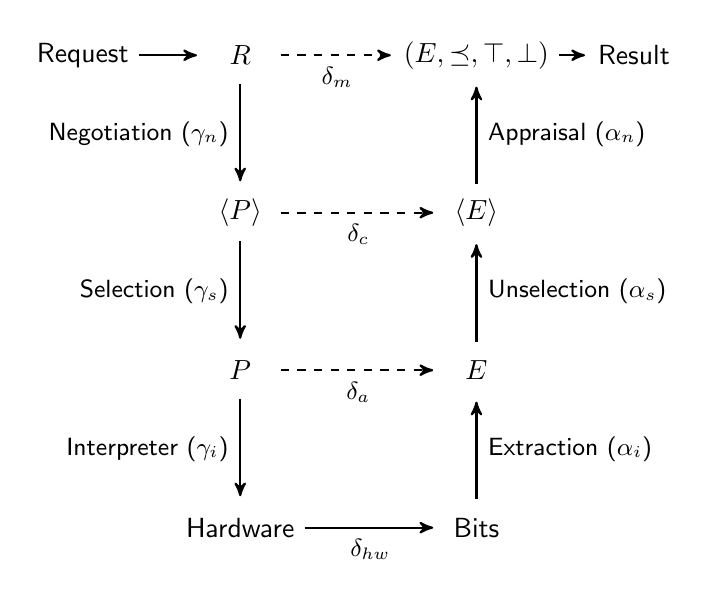
\begin{tikzpicture}[->,>=stealth',shorten >=1pt,auto,node distance=2.0cm,
  thick,main node/.style={rectangle,%%fill=blue!20,draw,
    font=\sffamily,minimum height=7mm,minimum width=10mm}]

  \node[main node] (NM) {$R$};
  \node[main node] (AM) [below of=NM] {$\langle P\rangle $};
  \node[main node] (CP) [below of=AM] {$P$};
  \node[main node] (HW) [below of=CP] {Hardware};
  \node[main node] (HWE) [node distance=3.0cm, right of=HW] {Bits};
  \node[main node] (CPE) [node distance=3.0cm, right of=CP] {$E$};
  \node[main node] (AME) [node distance=3.0cm, right of=AM] {$\langle E\rangle$};
  \node[main node] (NME) [node distance=3.0cm, right of=NM]
  {$(E,\preceq,\top,\bot)$};
  \node[main node] (IN) [node distance=2.0cm, left of=NM] {Request};
  \node[main node] (OUT) [node distance=2.0cm, right of=NME] {Result};
    

  \path[every node/.style={font=\sffamily\small, fill=white,inner sep=1pt}]
    (NM) edge [bend left=0] node[left=1mm] {Negotiation ($\gamma_{n}$)} (AM)
    (AM) edge [bend left=0] node[left=1mm] {Selection ($\gamma_{s}$)} (CP)
    (CP) edge [bend left=0] node[left=1mm] {Interpreter ($\gamma_{i}$)} (HW)
    (HW) edge node[below=1mm] {$\delta_{hw}$} (HWE)
    (CP) edge [dashed] node[below=1mm] {$\delta_a$} (CPE)
    (AM) edge [dashed] node[below=1mm] {$\delta_c$} (AME)
    (NM) edge [dashed] node[below=1mm] {$\delta_m$} (NME)
    (IN) edge (NM)
    (NME) edge (OUT)
    (HWE) edge node[right=1mm] {Extraction ($\alpha_i$)} (CPE)
    (CPE) edge node[right=1mm] {Unselection ($\alpha_s$)} (AME)
    (AME) edge node[right=1mm] {Appraisal ($\alpha_n$)} (NME)
    ;
\end{tikzpicture}

%%% Local Variables: 
%%% mode: latex
%%% TeX-master: "certification"
%%% End:

  \caption[Certification Figure]{Certification stack showing
    certification dependencies and execution path. Solid lines
    represent implementations while dashed lines represent
    mathematical definitions.}
  \label{fig:certification-fig}
\end{figure}

\section {Evidence}

Overall, the goal of Copland, and the precursor of negotiation is preforming
layered attestations.  The result of the layered attestation is to provide
an appraiser with evidence about the integrity of a target. 

\end{document}

